\documentclass{standalone}
\usepackage{amsmath}
\usepackage{tikz}

\begin{document}

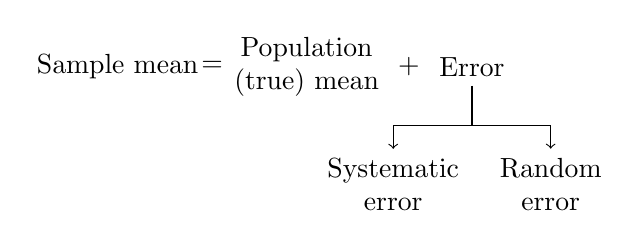
\begin{tikzpicture}
\node (samplemean) at (0,0) {Sample mean};
\node (equals) at (1.2,0) {=};
\node [align=center](populationmean) at (2.4,0) {Population \\ (true) mean};
\node (plus) at (3.7,0) {+};

\node (error) at (4.5,0) {Error};

\node[below of=error, align=center, xshift=-1cm, yshift=-0.5cm] (systematicerror) {Systematic \\ error};
\node[right of=systematicerror, align=center, xshift=1cm] (randomerror) {Random \\ error};

\draw[->] (error.south) -- ++(0,-0.5)-|  node[near start,below] {}(systematicerror.north);
\draw[->] 	(error.south)-- ++(0,-0.5)-| node[near start,below] {}(randomerror.north);
\end{tikzpicture}

\end{document}
